%!TEX root = pfc-memoria.tex
%!TEX encoding = UTF-8 Unicode

\chapter{Procesamiento del lenguaje natural}

\section{Lenguaje natural vs lenguajes formales}

\section{Preprocesamiento}

\subsection{\emph{``Tokenización''}}

La \emph{tokenización}\index{tokenización}\index{tokenization@\emph{tokenization}} en NLP es normalmente el proceso de separar la cadena de entrada, frases en lenguaje natural, en las distintas palabras que componen la frase. Puede ser simplemente un separador que trocee la frase cada vez que se encuentre un espacio.
\begin{listing}[H]
\begin{minted}{python}
>>> 'of escapades demonstrating the adage that what is good for the goose'.split()
['of', 'escapades', 'demonstrating', 'the', 'adage', 'that', 'what', 'is', 'good', 'for', 'the', 'goose']
>>> 
\end{minted}
\caption{Tokenización sencilla mediante la separación de espacios.}
\label{lst:tokenizacion-sencilla}
\end{listing}

La tokenización en su sentido más amplio y general es el procedimiento del análisis léxico para reconocer lexemas del flujo de entrada con la que se obtiene un flujo de salida compuesto por tokens \citep[§2.2]{Jimenez2004}.

\begin{definition}[Token] \index{token}
Denominamos \emph{token} al conjunto de cadenas de caracteres con significado mínimo.
\end{definition}

\begin{definition}[Patrón] \index{patrón}
El \emph{patrón} es una regla que describe el conjunto de caracteres que cuadran un token.
\end{definition}

El concepto de ``cuadrar'' se denomina en inglés como match\index{match@\emph{match}}, y también se puede traducir como concordancia o correspondencia.

\begin{definition}[Lexema] \index{lexema}
Un \emph{lexema} es una secuencia concreta de caracteres que se corresponde con el patrón de un token determinado.
\end{definition}

\begin{example} \index{token} \index{patrón} \index{lexema}
Pongamos algunos ejemplos de tokens, patrones y lexemas, de un lenguaje formal típico de programación:
\nopagebreak
\begin{center}
\begin{tabular}{|l|l|l|}
\hline
\textbf{token} & \textbf{lexemas de ejemplo} & \textbf{descripción informal del patrón} \\ \hhline{===}
\codep{CONST} & \codep{const} & const \\ \hline
\codep{IF} & \codep{if} & if \\ \hline
\codep{OPREL} & \codep{<}, \codep{<=}, \codep{=}, \codep{>}, \codep{>=} & <~ ó <= ó = ó >~ ó >= \\ \hline
\codep{ID} & \codep{pi}, \codep{contador}, \codep{D2} & letra seguida de letras y dígitos \\ \hline
\codep{CTENUM} & \codep{3.1416}, \codep{0}, \codep{6.1E23} & cualquier constante numérica \\ \hline
\codep{LITERAL} & \codep{"core dumped"} & cualesquiera letras entre \codep{"} y \codep{"} excepto \codep{"} \\ \hline
\end{tabular}
\end{center}
\end{example}

En lenguaje natural, la unidad mínima de información textual será la palabra. De manera que token y lexema coinciden siempre, y no tiene sentido definir un patrón para cada token de las palabras de un diccionario de la lengua, ya que el patrón es la propia secuencia de letras de la palabra.

Existen distintos niveles de tokenización de documentos \citep[ch.~1]{Perkins2010}:
\nopagebreak
\begin{itemize}
\item Tokenizar textos en frases.
\item Tokenizar frases en palabras.
\end{itemize}

Simplemente para la primera tarea ya nos encontramos con dificultades, pues las frases no sólo terminan en punto. Pueden terminar en punto (\codep{.}), signo de exclamación (\codep[text]{!}), signo de interrogación (\codep[text]{?}), en algunos casos dos puntos (\codep{:}). Y en otros idiomas, como el español, también hay que tener en cuenta que en la separación entre frases puede haber signos de apertura de interrogación o exclamación, etc. Y también hay que tener en cuenta los puntos que separan unidades de millar en una cifra, o los puntos suspensivos, los puntos usados en acrónimos y abreviaturas, \ldots, para no interpretarlo como separador de frases en estos casos.

En cuanto a la separación de palabras, también pueden surgir problemas, dependiendo del idioma. En el siguiente ejemplo (\autoref{lst:wordtokenizers}) podemos ver distintas formas de separar palabras de una frase en inglés que usa contracciones.\footnote{También se puede encontrar un demostrador interactivo de la tokenización en la siguiente dirección:\\
\url{http://text-processing.com/demo/tokenize/}}

\begin{listing}[H]
\begin{minted}{python}
>>> from nltk.tokenize import TreebankWordTokenizer, WordPunctTokenizer, WhitespaceTokenizer
>>> TreebankWordTokenizer().tokenize("Can't is a contraction.")
['Ca', "n't", 'is', 'a', 'contraction', '.']
>>> WordPunctTokenizer().tokenize("Can't is a contraction.")
['Can', "'", 't', 'is', 'a', 'contraction', '.']
>>> WhitespaceTokenizer().tokenize("Can't is a contraction.")
["Can't", 'is', 'a', 'contraction.']
>>> 
\end{minted}
\caption{Diferentes estrategias de separación de palabras}
\label{lst:wordtokenizers}
\end{listing}

Una mejor aproximación al problema es reemplazar --previamente a la tokenización--, las palabras contraídas con sus palabras equivalentes sin contracción.\footnote{Puede obtenerse un catálogo bastante extenso de contracciones en inglés --en uso y arcaicas--, en la dirección: \url{http://www.enchantedlearning.com/grammar/contractions/list.shtml}}
Para ello es necesario construirse una tabla que establezca el mapping \citep{Perkins2014}.

Como ejemplo de un conjunto de substitución, véase una tabla no exhaustiva en la \autoref{tbl:contracciones}, en dos versiones:
\nopagebreak
\begin{enumerate}[(a)]
\item En la primera de ellas se implementaría empleando un diccionario común de palabras de búsqueda y reemplazo, directamente.
\item En la segunda opción, se hace uso de expresiones regulares para condensar la tabla y no tener que hacer explícito todas las posibles contracciones que compartan sufijos sinónimos.
\end{enumerate}

\begin{table}[htbp]
\centering
\begin{subtable}[t]{0.45\linewidth}
\centering
\begin{tabular}{|l|l|}
\hline
\textbf{contracción} & \textbf{reemplazar con} \\ \hhline{==}
isn't & is not \\ \hline
aren't & are not \\ \hline
wasn't & was not \\ \hline
weren't & were not \\ \hline
haven't & have not \\ \hline
hasn't & has not \\ \hline
couldn't & could not \\ \hline
shouldn't & should not \\ \hline
mightn't & might not \\ \hline
mustn't & must not \\ \hline
could've & could have \\ \hline
might've & might have \\ \hline
must've & must have \\ \hline
ma'am & madam \\ \hline
she'd've & she would have \\ \hline
'tisn't & it is not \\ \hline
who'll & who will \\ \hline
when'll & when will \\ \hline
what're & what are \\ \hline
we're & we are \\ \hline
they're & they are \\ \hline
that's & that is \\ \hline
I'll & I will \\ \hline
you'll & you will \\ \hline
he'll & he will \\ \hline
she'll & she will \\ \hline
\end{tabular}
\caption{Sustitución literal}
\label{tbl:contracciones-directa}
\end{subtable}
\begin{subtable}[t]{0.45\linewidth}
\centering
\begin{tabular}{|l|l|}
\hline
\textbf{contracción} & \textbf{reemplazar con} \\ \hhline{==}
\verb=r"won't"= & \verb="will not"= \\ \hline
\verb=r"can't"= & \verb="cannot"= \\ \hline
\verb=r"i'm"= & \verb="i am"= \\ \hline
\verb=r"ain't"= & \verb="is not"= \\ \hline
\verb=r"(\w+)'ll"= & \verb="\g<1> will"= \\ \hline
\verb=r"(\w+)n't"= & \verb="\g<1> not"= \\ \hline
\verb=r"(\w+)'ve"= & \verb="\g<1> have"= \\ \hline
\verb=r"(\w+)'s"= & \verb="\g<1> is"= \\ \hline
\verb=r"(\w+)'re"= & \verb="\g<1> are"= \\ \hline
\verb=r"(\w+)'d"= & \verb="\g<1> would"= \\ \hline
\end{tabular}
\caption{Sustitución condensada mediante expresiones regulares}
\label{tbl:contracciones-regexp}
\end{subtable}
\vfill
\caption{Sustitución de contracciones en inglés}
\label{tbl:contracciones}
\end{table}

\subsection{Supresión de palabras vacías (\emph{stopwords})}

\ldots

\subsection{Radicación \emph{``Stemming''}}

La \emph{decodificación primaria}\index{decodificación primaria} es la herramienta instintiva que permite a los hablantes de un idioma intuir el significado de una palabra desconocida del idioma --siendo conocido el subconjunto común y más frecuente del mismo--, a partir de sus elementos léxicos \citep{Zubira2002}. Son tres:
\nopagebreak
\begin{description}
\item[La contextualización.]\index{contextualización} Por medio de este mecanismo rastreamos el significado de la palabra valiéndonos del contexto o entorno de las frases en las cuales está inscrita. Ejemplos:
\nopagebreak
\begin{itemize}
\item ``Lo admiran por su \textbf{sindéresis}, ya que su \emph{capacidad para juzgar} es notable.'' $\Longrightarrow$ El contexto nos permite deducir que el significado de sindéresis es la capacidad para juzgar.
\item ``Los \emph{derechos económicos, sociales y culturales} son de segundo orden. Los \textbf{DESC} suponen mayores demandas.'' $\Longrightarrow$ El contexto nos permite intuir que el acrónimo DESC se refiere a derechos económicos, sociales y culturales.
\end{itemize}
%
\item[La sinonimia.]\index{sinonimia} Mediante la sinonimia, se puede hacer coincidir el significado de la palabra desconocida con términos semejantes que se han mencionado antes de ella (anáfora) o que se mencionarán después (catáfora) en el texto. Ejemplo:
\nopagebreak
\begin{itemize}
\item ``Nadie ha visto al \textbf{abate}. Parece que este \emph{clérigo} ha desaparecido.'' $\Longrightarrow$ El sinónimo de abate es clérigo, aunque seguramente tenga algún matiz que lo convierte en un término con mayor especificidad.
\end{itemize}
%
\item[La radicación.]\index{radicación} En inglés \emph{stemming}\index{stemming@\emph{stemming}}. La radicación consiste en descomponer la palabra en sus elementos constituyentes o afijos: prefijos, infijos y sufijos. Ejemplos:\footnote{Pueden consultarse más ejemplos en \url{http://www.slideshare.net/sandracasierra/decodificacin-primaria}}
\nopagebreak
\begin{itemize}
\item \textbf{postdiluviano} $\Longrightarrow$ Después (post-) de un diluvio.
\item \textbf{subtropical}  $\Longrightarrow$ Por debajo (sub-) del trópico.
\end{itemize}
\end{description}

La manera más común de realizar la radicación\index{radicación}\index{stemming@\emph{stemming}} en aplicaciones de NLP es eliminar los sufijos para quedarse con la raíz de la palabra, y su significado más primitivo (véase \autoref{lst:PorterStemmer}).

\begin{listing}[htbp]
\begin{minted}{python}
>>> from nltk.stem import PorterStemmer
>>> stemmer = PorterStemmer()
>>> stemmer.stem('cookery')
'cookeri'
>>> stemmer.stem('cooking')
'cook'
>>> stemmer.stem('series')
'seri'
>>> stemmer.stem('women')
'women'
>>> stemmer.stem('riding')
'ride'
>>> 
\end{minted}
\caption{Funcionamiento de \codep{PorterStemmer}}
\label{lst:PorterStemmer}
\end{listing}

\codep{PorterStemmer} es la implementación en NLTK del algoritmo de radicación de Martin Porter \citep{Porter1980}. Es un algoritmo --muy usado para lengua inglesa--, de eliminación o reemplazo de sufijos en varias iteraciones.

Aunque se pierda algo de información, tiene sus ventajas:
\nopagebreak
\begin{itemize}
\item Sirve para reducir el tamaño del vocabulario; y por consiguiente, el orden del tiempo y el espacio que ocupan los programas de procesamiento.
\item Sirve para asemejar conceptos similares, que es normalmente lo deseable al hacer una búsqueda o extracción de información.
\item También sirve para acelerar el procesamiento y reducir el tamaño de los índices de los motores de búsqueda.
\end{itemize}

No obstante también tiene alguna desventaja:
\nopagebreak
\begin{itemize}
\item Al estar basado en la eliminación literal de sufijos, puede producir palabras no válidas del idioma (como en \codep{'cookeri'} en el ejemplo anterior).
\end{itemize}

NLTK proporciona otros stemmers adicionales a \codep{PorterStemmer}:
\begin{description}
\item[\codep{LancasterStemmer}] Desarrollado en la Universidad de Lancaster, es ligeramente más agresivo que el algoritmo de Porter, aunque no existen estudios que confirmen la supremacía de uno sobre el otro \citep{Perkins2014}.
\item[\codep{RegexpStemmer}] Stemmer al que se puede recurrir para eliminar prefijos o sufijos de manera personalizada configurado mediante una expresión regular.
\item[\codep{SnowballStemmer}] Snowball extiende el método Porter para su aplicación a otros idiomas indoeuropeos: románicos, germánicos y escandinavos.
\end{description}

\subsection{Lematización}

La lematización\index{lematización} (\emph{lemmatizing}\index{lemmatizing@\emph{lemmatizing}} en inglés) es el proceso lingüístico que sustituye una palabra con forma \emph{flexionada} (plural, femenino, verbo conjugado, \ldots) por su \textbf{lema}. Tiene el mismo objetivo que la radicación, pero a diferencia de aquel, la lematización siempre produce una palabra válida en el idioma.
\begin{definition}[Lema]
En lingüística, el \emph{lema}\index{lema} es la forma que por convenio se acepta como representante de todas las formas flexionadas de una misma palabra.
\end{definition}

\subsection{Anotación gramatical de la parte de la oración (\emph{Part-of-speech tagging}) }

En gramática tradicional, la clasificación según categorías gramaticales es de tipo semántico y no funcional. En la gramática española el término fue introducido por Antonio de Nebrija \citep[Categoría gramatical]{wikipedia-es}. La gramática tradicional distingue nueve partes de la oración\index{parte de la oración}\index{part-of-speech@\emph{part-of-speech}} (las ocho de Nebrija más el artículo):
\nopagebreak
\begin{enumerate}
\item Artículo o determinante
\item Sustantivo o nombre
\item Pronombre
\item Verbo
\item Adjetivo
\item Adverbio
\item Preposición
\item Conjunción
\item Interjección
\end{enumerate}

El proceso de anotación gramatical POS convierte la lista de palabras, en una lista de pares de palabras con su etiqueta POS indicando si funciona como nombre, verbo, adjetivo, \ldots

En NLTK existen diversos \emph{taggers}\index{POS tagger@\emph{POS tagger}}, y pueden combinarse en una cadena de taggers de manera que si uno no es capaz de asignar la etiqueta sin ambigüedad, se intenta con el siguiente en la cadena.

En los taggers se pueden establecer reglas que permitan identificar la parte de la oración de la palabra a partir de su lexicografía, o bien teniendo en cuenta el contexto (un número de palabras anteriores). Por ejemplo: si sólo vemos la palabra \codep{'la'}, podemos suponer que se trata del artículo determinado femenino singular, que es lo más común; mientras que si tenemos en cuenta la palabra en su contexto: \codep{'la sigue a sol en la escala de notas musicales'}, la palabra \codep{'la'} funciona como sustantivo al ser el nombre de una nota musical.

Para estos casos, el tagger dependiente del contexto se entrena mediante alguna técnica de aprendizaje automático sobre un corpus previamente anotado manualmente. De este entrenamiento, el tagger extrae la reglas de prelación, o realiza la inferencia estadística que le permita identificarlo correctamente para la mayoría de los casos. Evidentemente, funcionará mejor cuando el texto a anotar sea del mismo dominio del lenguaje que el texto usado para el entrenamiento.

También existen distintos conjuntos de etiquetas posibles, dependiendo del autor y del idioma a anotar. En la \autoref{tbl:pos-tags} se muestran (a) los que se utilizan en el proyecto Penn Treebank de la Universidad de Pennsylvania,\footnote{Extraído de \url{http://www.ling.upenn.edu/courses/Fall_2003/ling001/penn_treebank_pos.html}} (b) la correspondencia con los tags del corpus de WordNet.

\begin{table}[htbp]
\centering
\begin{subtable}[t]{0.60\linewidth}
\centering
\begin{tabular}{|l|l|l|}
\hline
\textbf{\#} & \textbf{tag} & \textbf{descripción} \\ \hhline{===}
1 & \verb=CC= & Coordinating conjunction \\ \hline
2 & \verb=CD= & Cardinal number \\ \hline
3 & \verb=DT= & Determiner \\ \hline
4 & \verb=EX= & Existential \emph{there} \\ \hline
5 & \verb=FW= & Foreign word \\ \hline
6 & \verb=IN= & Preposition or subordinating conjunction \\ \hline
7 & \verb=JJ= & Adjective \\ \hline
8 & \verb=JJR= & Adjective, comparative \\ \hline
9 & \verb=JJS= & Adjective, superlative \\ \hline
10 & \verb=LS= & List item marker \\ \hline
11 & \verb=MD= & Modal \\ \hline
12 & \verb=NN= & Noun, singular or mass \\ \hline
13 & \verb=NNS= & Noun, plural \\ \hline
14 & \verb=NNP= & Proper noun, singular \\ \hline
15 & \verb=NNPS= & Proper noun, plural \\ \hline
16 & \verb=PDT= & Predeterminer \\ \hline
17 & \verb=POS= & Possessive ending \\ \hline
18 & \verb=PRP= & Personal pronoun \\ \hline
19 & \verb=PRP$= & Possessive pronoun \\ \hline
20 & \verb=RB= & Adverb \\ \hline
21 & \verb=RBR= & Adverb, comparative \\ \hline
22 & \verb=RBS= & Adverb, superlative \\ \hline
23 & \verb=RP= & Particle \\ \hline
24 & \verb=SYM= & Symbol \\ \hline
25 & \verb=TO= & \emph{to} \\ \hline
26 & \verb=UH= & Interjection \\ \hline
27 & \verb=VB= & Verb, base form \\ \hline
28 & \verb=VBD= & Verb, past tense \\ \hline
29 & \verb=VBG= & Verb, gerund or present participle \\ \hline
30 & \verb=VBN= & Verb, past participle \\ \hline
31 & \verb=VBP= & Verb, non-3rd person singular present \\ \hline
32 & \verb=VBZ= & Verb, 3rd person singular present \\ \hline
33 & \verb=WDT= & Wh-determiner \\ \hline
34 & \verb=WP= & Wh-pronoun \\ \hline
35 & \verb=WP$= & Possessive wh-pronoun \\ \hline
36 & \verb=WRB= & Wh-adverb \\ \hline
\end{tabular}
\caption{POS tags del Penn Treebank}
\label{tbl:pos-tags-peen-treebank}
\end{subtable}
\begin{subtable}{0.38\linewidth}
\centering
\begin{tabular}{|l|l|}
\hline
\textbf{WordNet} & \textbf{Treebank} \\ \hhline{==}
n & NN \\ \hline
a & JJ \\ \hline
s & JJ \\ \hline
r & RB \\ \hline
v & VB \\ \hline
\end{tabular}
\caption{POS tags correspondientes en WordNet}
\label{tbl:pos-tags-wordnet}
\end{subtable}
\caption{Etiquetas POS en Penn Treebank y en WordNet}
\label{tbl:pos-tags}
\end{table}

\subsection{Resumen de procedimientos de preprocesamiento}

\begin{figure}[H]
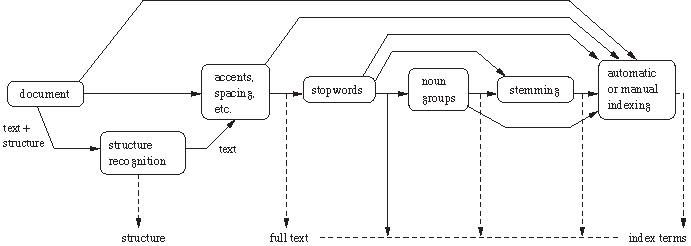
\includegraphics[width=0.98\textwidth]{procesamiento-textos-mod-ir}
\caption[Resumen de procedimientos de preprocesamiento]{Resumen de procedimientos de preprocesamiento \citep[ch. 7]{Baeza-Yates2011}}
\end{figure}

\section{Análisis sintáctico}

\section{Modelo de espacio vectorial semántico}

Se han usado espacios vectoriales para modelar la semántica de las palabras. A cada palabra del vocabulario se le asigna un vector $n$-dimensional, y es un hecho que este vector puede representar de alguna manera el significado de la palabra \citep{Socher2012}.

Después de realizar un entrenamiento en un gran corpus y usando un espacio vectorial de grandes dimensiones. Cuando converge, se observa que palabras con significado similar les corresponden vectores cercanos (en términos de la distancia coseno entre ellos). Por ejemplo, «powerful» y «strong» están cercanos, mientras que «powerful» y «Paris» no lo están. Incluso las operaciones algebraicas entre vectores semánticos también incorporan significado, de manera que puede responder a cuestiones por analogía:
$\text{«king»} - \text{«man»} + \text{«woman»} \approx \text{«queen»}$
\citep{DBLP:journals/corr/LeM14}.
